\documentclass[14pt]{beamer}
\usetheme{EastLansing}
\usecolortheme{spruce}

\usepackage{xcolor}
\usepackage{listings}
\usepackage{courier}
\usepackage{graphicx}
\usepackage{amsmath}
\usepackage{algorithm2e}
\usepackage[font=small]{caption}

\usefonttheme[onlymath]{serif}


\definecolor{mGreen}{rgb}{0,0.6,0}
\definecolor{mGray}{rgb}{0.5,0.5,0.5}
\definecolor{mPurple}{rgb}{0.8,0,0.82}
\definecolor{backgroundColour}{rgb}{0.95,0.95,0.92}
\definecolor{lightBlue}{rgb}{0.1, 0.1, 0.8}

\lstdefinestyle{CStyle}{
    backgroundcolor=\color{backgroundColour},   
    commentstyle=\color{mGreen},
    keywordstyle=\color{magenta},
    numberstyle=\tiny\color{mGray},
    stringstyle=\color{mPurple},
    basicstyle=\ttfamily\footnotesize,
    breakatwhitespace=false,         
    breaklines=true,                 
    captionpos=b,                    
    keepspaces=true,                 
    numbers=left,                    
    numbersep=5pt,                  
    showspaces=false,                
    showstringspaces=false,
    showtabs=false,                  
    tabsize=2,
    language=C
}

\lstdefinestyle{pseudo}{
        basicstyle=\ttfamily\footnotesize,
        keywordstyle=\color{lightBlue},
        morekeywords={BEGIN,END,IF,ELSE,ENDIF,PRINT,WHILE,RETURN},
        morecomment=[l]{//},
        commentstyle=\color{mGreen},
        tabsize=2
}

\lstset{basicstyle=\footnotesize\ttfamily,breaklines=true}
\lstset{framextopmargin=50pt,tabsize=4}

\title{ELEC3850 - Embedded Systems 1}
\subtitle{STM32 I/O\\Interrupts}
\author{Brenton Schulz}
\institute{University of Newcastle}
\date{\today}

\begin{document}
\titlepage

\begin{frame}
\frametitle{Summary}
\begin{itemize}
\item Software driven GPIO
\item Peripherals
	\begin{itemize}
		\item SPI
		\item I2C
		\item UART
	\end{itemize}
\item Interrupts
\end{itemize}
\end{frame}

\begin{frame}[fragile]
\frametitle{Levels of Understanding}
\begin{itemize}
\item Fundamental electronics
	\begin{itemize}
		\item Transistors drive pins
		\item What is push-pull Vs. open drain?
		\item What are "pull-ups"?
	\end{itemize}
\item Datasheet / reference manual
	\begin{itemize}
		\item Low-level configuration registers drive the GPIO circuit
	\end{itemize}
\item CubeMX
	\begin{itemize}
		\item How does the datasheet translate to CubeMX?
		\item In general: CubeMX assumes you have read the reference manual
	\end{itemize}
\item HAL
	\begin{itemize}
		\item Using the HAL with confidence requires an understanding over everything above
	\end{itemize}
\end{itemize}
\end{frame}

\begin{frame}[fragile]
\frametitle{GPIO Hardware}
\begin{center}
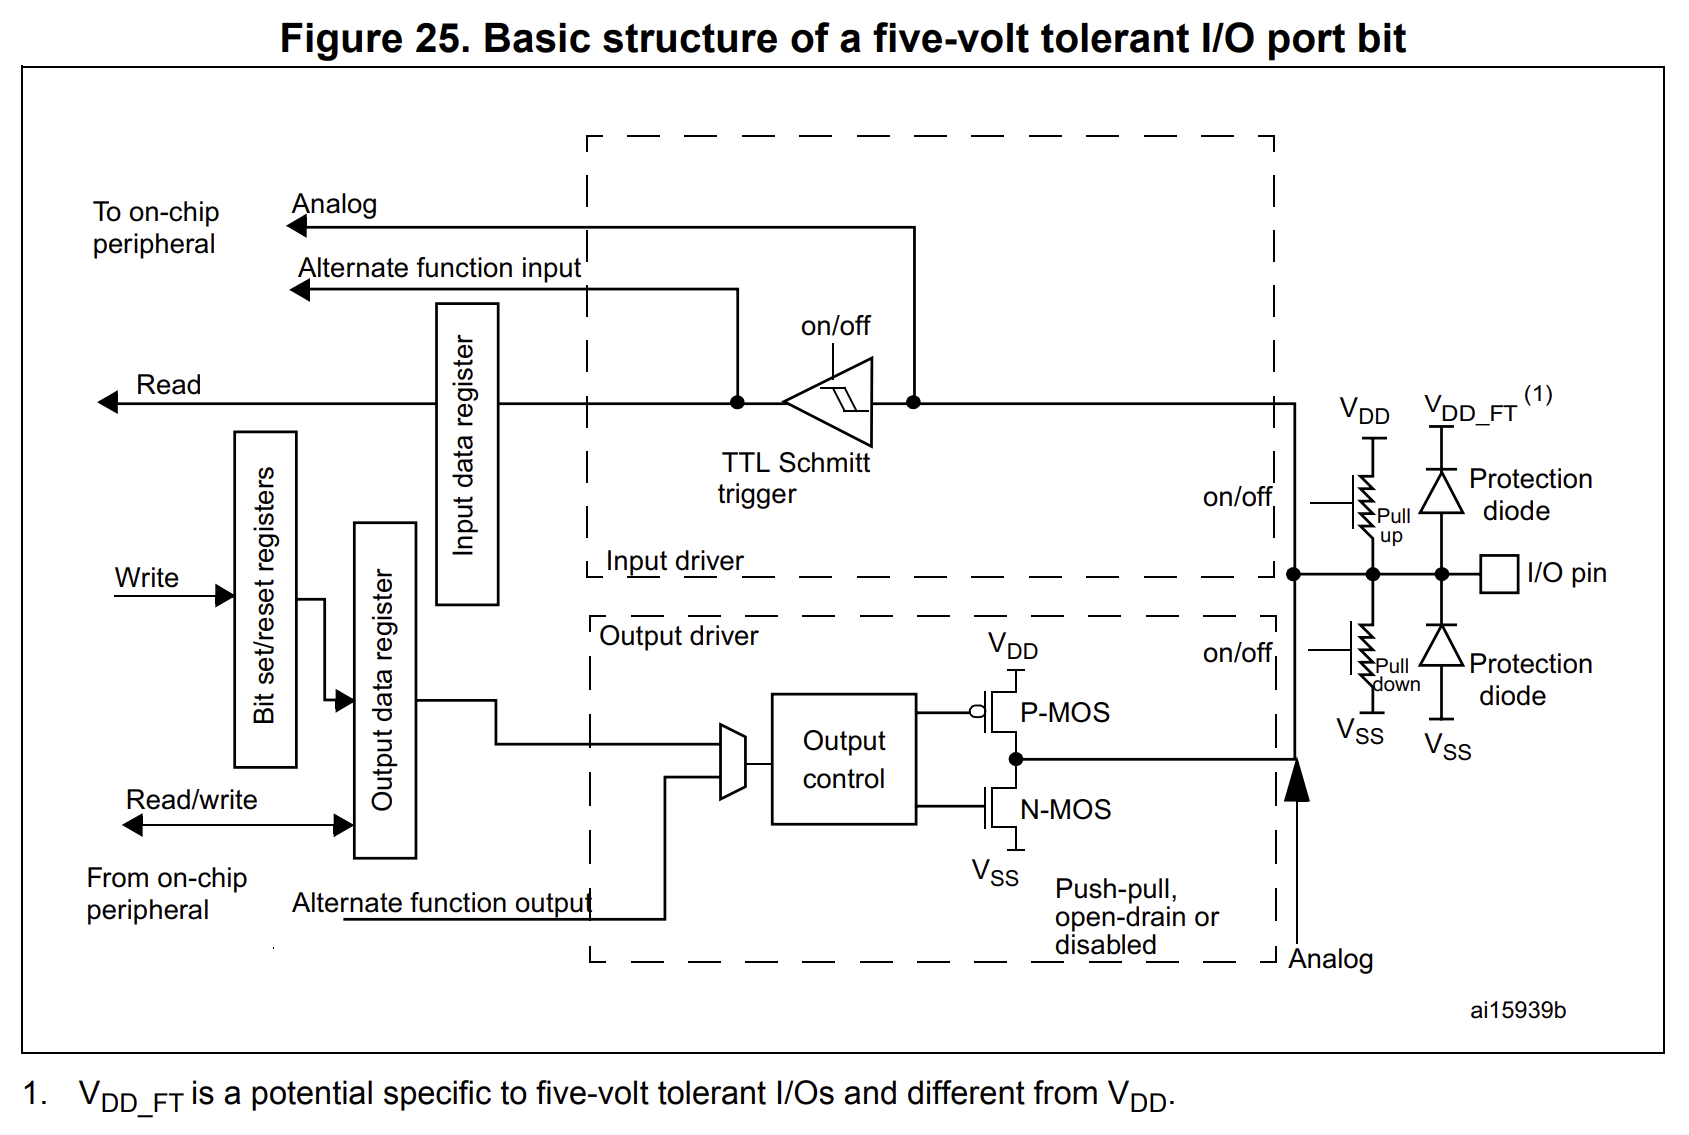
\includegraphics[width=0.9\framewidth]{gpio}
\end{center}
\end{frame}

\begin{frame}[fragile]
\frametitle{GPIO Hardware}
\begin{itemize}
\item STM32 pins can be configured as:
	\begin{itemize}
		\item Digital outputs
			\begin{itemize}
				\item Push-pull
				\item Open drain
			\end{itemize}
		\item Digital inputs
			\begin{itemize}
				\item With or without pull-up
				\item With or without pull-down
			\end{itemize}
		\item Alternate Function I/Os
			\begin{itemize}
				\item Outputs can also push-pull or open drain
				\item AF inputs are analog when they drive internal ADCs
			\end{itemize}
	\end{itemize}
\item STM32 outputs also have output bandwidth control
\item NB: Outputs can have pull up/down enabled
	\begin{itemize}
		\item This wastes a small amount of power
		\item Useful if a pin swaps between input and output
	\end{itemize}
\end{itemize}
\end{frame}

\begin{frame}[fragile]
\frametitle{GPIO Control Bits}
\begin{center}
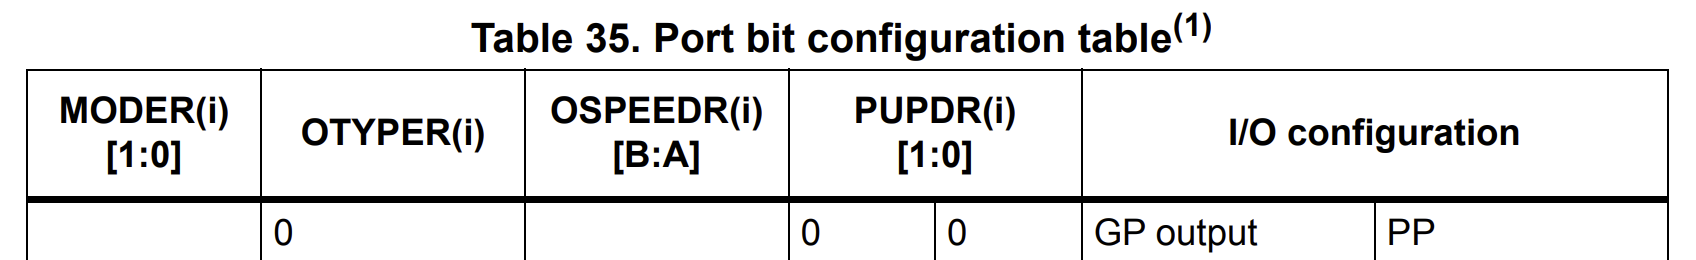
\includegraphics[width=0.9\framewidth]{gpioBits}
\end{center}
\begin{itemize}
\item Control bits:
	\begin{itemize}
		\item MODER - Input/output control
		\item OTYPER - Push-pull or open drain
		\item OSPEEDR - Output bandwidth limiting
		\item PUPDR - Pull up/down enable bits
	\end{itemize}
\item These control bits are packed into 32-bit GPIO registers:
	\begin{itemize}
		\item GPIOx\_MODER
		\item GPIOx\_OTYPER
		\item GPIOx\_OSPEEDR
		\item GPIOx\_PUPDR
	\end{itemize}
\end{itemize}
\end{frame}

\begin{frame}[fragile]
\frametitle{CubeMX}
\begin{itemize}
\item To configure GPIOs in CubeMX click pins and select a mode:
\begin{center}
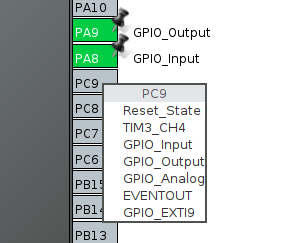
\includegraphics[width=0.3\framewidth]{gpio1}
\end{center}

\item Pull mode is then found in the left panel:
\begin{center}
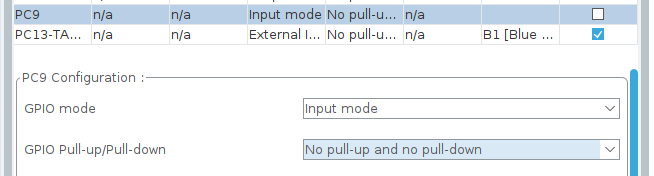
\includegraphics[width=0.7\framewidth]{gpio2}
\end{center}

\end{itemize}
\end{frame}

\begin{frame}[fragile]
\frametitle{HAL Translation}
\begin{itemize}
\item Open STM32CubeIDE, perform example configuration
\item Observe:
	\begin{itemize}
		\item \texttt{GPIO\_TypeDef} - compare to GPIO registers in reference manual
		\item \texttt{HAL\_GPIO\_*} functions in \texttt{stm32f4xx\_hal\_gpio.h}
		\item HAL \texttt{GPIO\_PinState} datatype
	\end{itemize}
\end{itemize}
\end{frame}

\begin{frame}[fragile]
\frametitle{Interrupts Review}
\begin{itemize}
\item An \textit{interrupt} is an event which causes the CPU to:
\begin{itemize}
\item Stop what it was doing
\item Execute an \textit{interrupt service routine} (ISR)
\item Resume what it was doing
\end{itemize}
\item An ISR is a C function with a specific name
	\begin{itemize}
		\item These names are listed in the HAL in \texttt{startup\_xxx.s}
		\item The memory locations of the ISRs get packed into the interrupt vector table - at the start of program memory on an ARM CPU
		\item By default ISRs are declared \texttt{weak} so you can define your own versions without removing the ``default`` versions
	\end{itemize}
\end{itemize}
\end{frame}

\begin{frame}[fragile]
\frametitle{Interrupts Review}
\begin{itemize}
\item ARM CPUs use a nested vector interrupt controller (NVIC) to control the interrupt process
\item The \textit{nested} behaviour is the ability of interrupts to trigger (and their ISRs execute) while another ISR is already executing
	\begin{itemize}
		\item Interrupts have \textit{priorities} which control when they can preempt each other
	\end{itemize}
\item The ``vector'' term relates to ISRs having unique program memory addresses which are jumped to when an interrupt triggers
\end{itemize}
\end{frame}

\begin{frame}[fragile]
\frametitle{GPIO Interrupts}
\begin{itemize}
\item STM32s can have interrupts triggered by GPIO state changes:
	\begin{itemize}
		\item Rising
		\item Falling
		\item Both
	\end{itemize}
\item There are 16 GPIO external interrupt (\texttt{EXTI}) sources on most STM32s
	\begin{itemize}
		\item Each can be triggered off 1 GPIO pin as-per Figure 42, p382 of RM0090
		\item tl;dr: \texttt{PORT}xN triggers \texttt{EXTI}N
			\begin{itemize}
				\item eg: PORTB2 can trigger EXTI2
			\end{itemize}
	\end{itemize}
\end{itemize}
\end{frame}

\begin{frame}[fragile]
\frametitle{GPIO Interrupts}
\begin{itemize}
\item The possible interrupt vectors are:
	\begin{itemize}
		\item EXTI0
		\item EXTI1
		\item EXTI2
		\item EXTI3
		\item EXTI4
		\item EXTI9\_5
		\item EXTI10\_15
	\end{itemize}
\item ie: GPIO pins 0-4 have unique interrupts, the others trigger a ``grouped'' interrupt
	\begin{itemize}
		\item The ISR needs to determine which pin triggered the interrupt
	\end{itemize}
\end{itemize}
\end{frame}

\begin{frame}[fragile]
\frametitle{GPIO Interrupts}
\begin{itemize}
\item To use an external GPIO interrupt:
	\begin{enumerate}
		\item Configure the pin as EXTI in CubeMX
		\item Write the ISR function
		\item (Optional) Set the interrupt priority
			\begin{itemize}
				\item This is a big topic - not covered in this lecture
			\end{itemize}
		\item Enable the interrupt
	\end{enumerate}
\end{itemize}
\end{frame}

\begin{frame}[fragile]
\frametitle{GPIO Interrupts - Demonstration}
\begin{itemize}
\item Observe Nucleo-F103RB project
\item Note it includes \texttt{EXTI15\_10\_IRQHandler()}
	\begin{itemize}
		\item It did once then disappeared - CubeMX is weird
	\end{itemize}
\item This function, in turn, calls \texttt{HAL\_GPIO\_EXTI\_IRQHandler(GPIO\_PIN\_13)}
\begin{itemize}
	\item The HAL includes other interrupt functions with various names - these are \textbf{NOT} interrupt service routines called by the NVIC
\end{itemize}
\item If the \texttt{EXTI*\_IRQHandler()} function does not exist you need to write it
	\begin{itemize}
		\item It is the function \textit{actually called} by the NVIC when the interrupt triggers
	\end{itemize}
\end{itemize}
\end{frame}

\begin{frame}[fragile]
\frametitle{GPIO Interrupts}
\begin{itemize}
\item Very few interrupts are enabled by default!
\item Enable interrupts with \texttt{HAL\_NVIC\_EnableIRQ()}
	\begin{itemize}
		\item eg: \texttt{HAL\_NVIC\_EnableIRQ(EXTI15\_10\_IRQn)}
	\end{itemize}
\end{itemize}
\end{frame}

\begin{frame}[fragile]
\frametitle{GPIO Interrupts - Demonstration}
\begin{itemize}
\item Crucial note 2: EXTIs are not cleared by hardware!
\begin{itemize}
\item Software must clear the appropriate interrupt flag by writing a 1 to the correct bit in \texttt{EXTI\_PI}
\item Recommended to use \texttt{\_\_HAL\_GPIO\_EXTI\_CLEAR\_IT(GPIO\_PIN);}
\end{itemize}
\item Crucial note 3: When using shared EXTI interrupts use \texttt{\_\_HAL\_GPIO\_EXTI\_GET\_IT(GPIO\_PIN)} to test which EXTI triggered the ISR
\item \texttt{stm32f1xx\_hal\_gpio.h} must be included for both the macro and \texttt{GPIO\_PIN} definitions
\end{itemize}
\end{frame}

\begin{frame}[fragile]
\frametitle{UART}
\begin{itemize}
\item Review
\begin{itemize}
\item The UART is a serial communications device
\item It is \textit{asynchronous} - only a data signal is sent
	\begin{itemize}
		\item The clock rate is configured at sender and receiver
		\item The start of a transmission is synchronised with a ``start bit''
	\end{itemize}
\item UARTs are \textit{byte oriented} - they send or receive 8-bits
\end{itemize}
\item Demonstration: Configuration of a UART and code required to use \texttt{printf()} on a NUCLEO-F103RB
\item NB: STM32s contain UARTs and USARTs - the synchronous USART hardware can be configured with a clock pin but that will not be demonstrated here
\end{itemize}
\end{frame}

\begin{frame}[fragile]
\frametitle{UART - CubeMX Configuration}
\begin{itemize}
\item Creating a project with the NUCLEO-F103RB automatically configures USART2 for pins PA2 (Tx) and PA3 (Rx)
	\begin{itemize}
		\item These pins are connected to a virtual COM port on the ST-Link debugger - other boards may require a USB to UART adapter
	\end{itemize}
\end{itemize}
\end{frame}

\begin{frame}[fragile]
\frametitle{UART - libc}
\begin{itemize}
\item Low level \textit{system calls} needs to be written to handle data reads and writes
\item The \texttt{newlib} embedded version of \texttt{glibc} contains \texttt{printf()}
\item \texttt{printf()} eventually calls \texttt{\_\_io\_putchar()} to write characters
\item \texttt{\_\_io\_putchar()} is declared \texttt{weak} in \texttt{syscalls.c} - we need to write our own
	\begin{itemize}
		\item You can also write a \texttt{\_\_io\_putchar()} version which prints to other hardware, such as an LCD screen, i2c peripheral, etc
	\end{itemize}
\end{itemize}
\end{frame}

\begin{frame}[fragile]
\frametitle{UART - libc}
\begin{itemize}
\item We will write \texttt{\_\_io\_putchar()} to write characters to the USART2
\item This will use \texttt{HAL\_UART\_Transmit()}
	\begin{itemize}
		\item \texttt{HAL\_UART\_Transmit()} is \textit{blocking} - it won't return until data has been sent
		\item Non-blocking and interrupt-driven methods use far less CPU time
	\end{itemize}
\end{itemize}
\end{frame}

\end{document}
